% Created by tikzDevice version 0.12.5 on 2023-10-14 23:39:34
% !TEX encoding = UTF-8 Unicode
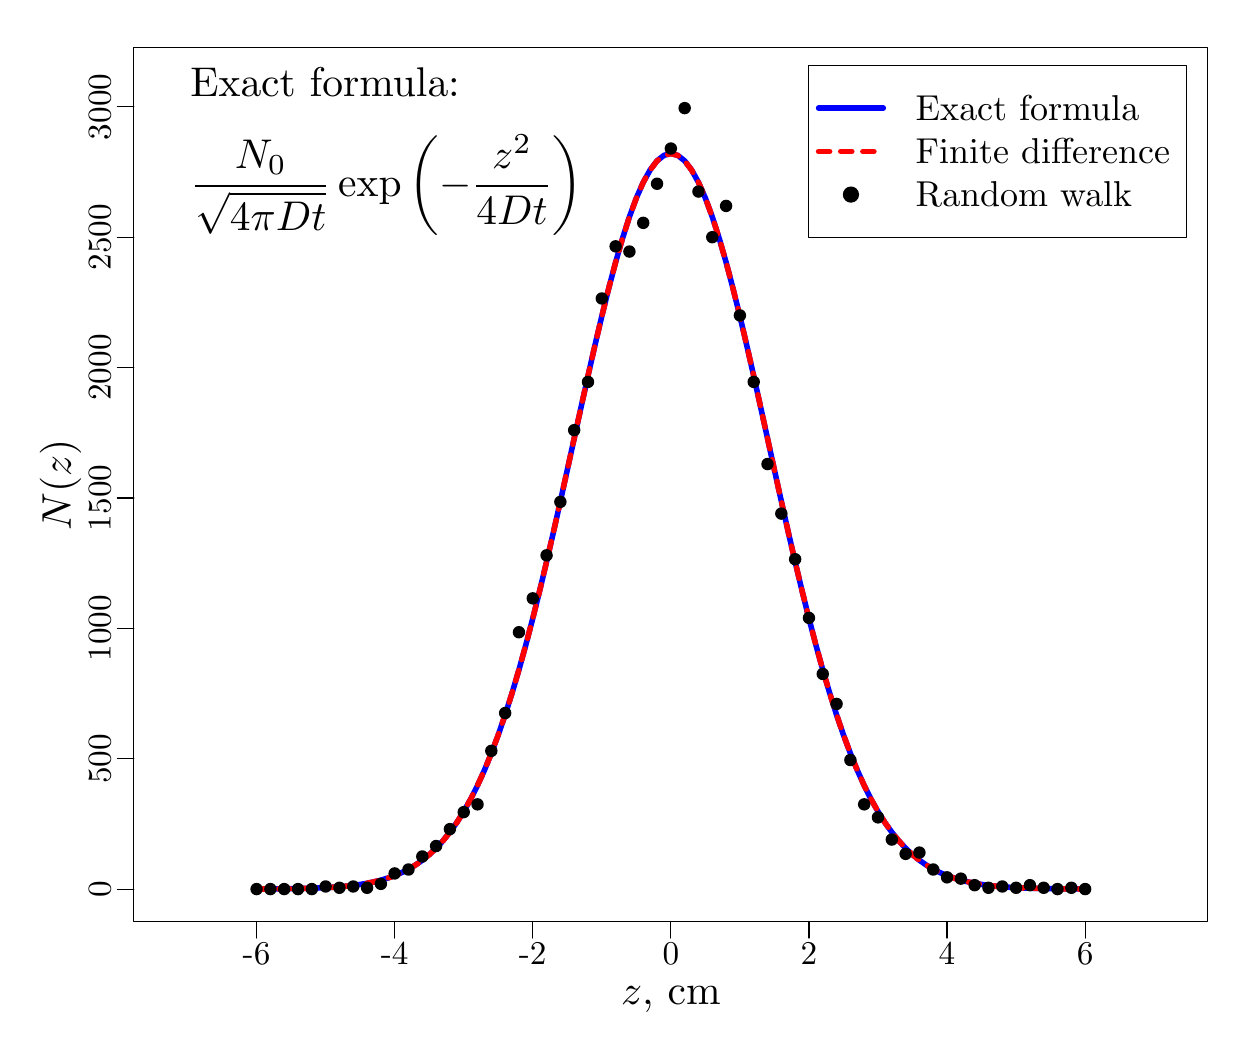
\begin{tikzpicture}[x=1pt,y=1pt]
\definecolor{fillColor}{RGB}{255,255,255}
\path[use as bounding box,fill=fillColor,fill opacity=0.00] (0,0) rectangle (433.62,361.35);
\begin{scope}
\path[clip] ( 38.40, 38.40) rectangle (426.42,354.15);
\definecolor{drawColor}{RGB}{0,0,255}

\path[draw=drawColor,line width= 2.0pt,line join=round,line cap=round] ( 82.71, 50.11) --
	( 85.21, 50.12) --
	( 87.70, 50.14) --
	( 90.20, 50.16) --
	( 92.69, 50.18) --
	( 95.19, 50.22) --
	( 97.68, 50.26) --
	(100.18, 50.32) --
	(102.67, 50.39) --
	(105.17, 50.48) --
	(107.66, 50.59) --
	(110.16, 50.74) --
	(112.65, 50.92) --
	(115.15, 51.14) --
	(117.64, 51.42) --
	(120.14, 51.76) --
	(122.63, 52.18) --
	(125.13, 52.69) --
	(127.62, 53.31) --
	(130.12, 54.06) --
	(132.61, 54.95) --
	(135.11, 56.01) --
	(137.60, 57.27) --
	(140.10, 58.75) --
	(142.59, 60.49) --
	(145.09, 62.51) --
	(147.58, 64.85) --
	(150.08, 67.55) --
	(152.57, 70.63) --
	(155.07, 74.13) --
	(157.56, 78.09) --
	(160.06, 82.55) --
	(162.55, 87.52) --
	(165.05, 93.04) --
	(167.54, 99.12) --
	(170.04,105.79) --
	(172.53,113.05) --
	(175.03,120.91) --
	(177.52,129.34) --
	(180.02,138.34) --
	(182.51,147.86) --
	(185.01,157.88) --
	(187.50,168.32) --
	(190.00,179.13) --
	(192.49,190.23) --
	(194.99,201.53) --
	(197.48,212.91) --
	(199.98,224.29) --
	(202.47,235.52) --
	(204.97,246.50) --
	(207.46,257.08) --
	(209.96,267.15) --
	(212.45,276.58) --
	(214.95,285.23) --
	(217.44,293.00) --
	(219.94,299.77) --
	(222.43,305.46) --
	(224.93,309.96) --
	(227.42,313.23) --
	(229.92,315.21) --
	(232.41,315.88) --
	(234.90,315.21) --
	(237.40,313.23) --
	(239.89,309.96) --
	(242.39,305.46) --
	(244.88,299.77) --
	(247.38,293.00) --
	(249.87,285.23) --
	(252.37,276.58) --
	(254.86,267.15) --
	(257.36,257.08) --
	(259.85,246.50) --
	(262.35,235.52) --
	(264.84,224.29) --
	(267.34,212.91) --
	(269.83,201.53) --
	(272.33,190.23) --
	(274.82,179.13) --
	(277.32,168.32) --
	(279.81,157.88) --
	(282.31,147.86) --
	(284.80,138.34) --
	(287.30,129.34) --
	(289.79,120.91) --
	(292.29,113.05) --
	(294.78,105.79) --
	(297.28, 99.12) --
	(299.77, 93.04) --
	(302.27, 87.52) --
	(304.76, 82.55) --
	(307.26, 78.09) --
	(309.75, 74.13) --
	(312.25, 70.63) --
	(314.74, 67.55) --
	(317.24, 64.85) --
	(319.73, 62.51) --
	(322.23, 60.49) --
	(324.72, 58.75) --
	(327.22, 57.27) --
	(329.71, 56.01) --
	(332.21, 54.95) --
	(334.70, 54.06) --
	(337.20, 53.31) --
	(339.69, 52.69) --
	(342.19, 52.18) --
	(344.68, 51.76) --
	(347.18, 51.42) --
	(349.67, 51.14) --
	(352.17, 50.92) --
	(354.66, 50.74) --
	(357.16, 50.59) --
	(359.65, 50.48) --
	(362.15, 50.39) --
	(364.64, 50.32) --
	(367.14, 50.26) --
	(369.63, 50.22) --
	(372.13, 50.18) --
	(374.62, 50.16) --
	(377.12, 50.14) --
	(379.61, 50.12) --
	(382.11, 50.11);
\end{scope}
\begin{scope}
\path[clip] (  0.00,  0.00) rectangle (433.62,361.35);
\definecolor{drawColor}{RGB}{0,0,0}

\path[draw=drawColor,line width= 0.4pt,line join=round,line cap=round] ( 82.71, 38.40) -- (382.11, 38.40);

\path[draw=drawColor,line width= 0.4pt,line join=round,line cap=round] ( 82.71, 38.40) -- ( 82.71, 32.40);

\path[draw=drawColor,line width= 0.4pt,line join=round,line cap=round] (132.61, 38.40) -- (132.61, 32.40);

\path[draw=drawColor,line width= 0.4pt,line join=round,line cap=round] (182.51, 38.40) -- (182.51, 32.40);

\path[draw=drawColor,line width= 0.4pt,line join=round,line cap=round] (232.41, 38.40) -- (232.41, 32.40);

\path[draw=drawColor,line width= 0.4pt,line join=round,line cap=round] (282.31, 38.40) -- (282.31, 32.40);

\path[draw=drawColor,line width= 0.4pt,line join=round,line cap=round] (332.21, 38.40) -- (332.21, 32.40);

\path[draw=drawColor,line width= 0.4pt,line join=round,line cap=round] (382.11, 38.40) -- (382.11, 32.40);

\node[text=drawColor,anchor=base,inner sep=0pt, outer sep=0pt, scale=  1.20] at ( 82.71, 22.80) {-6};

\node[text=drawColor,anchor=base,inner sep=0pt, outer sep=0pt, scale=  1.20] at (132.61, 22.80) {-4};

\node[text=drawColor,anchor=base,inner sep=0pt, outer sep=0pt, scale=  1.20] at (182.51, 22.80) {-2};

\node[text=drawColor,anchor=base,inner sep=0pt, outer sep=0pt, scale=  1.20] at (232.41, 22.80) {0};

\node[text=drawColor,anchor=base,inner sep=0pt, outer sep=0pt, scale=  1.20] at (282.31, 22.80) {2};

\node[text=drawColor,anchor=base,inner sep=0pt, outer sep=0pt, scale=  1.20] at (332.21, 22.80) {4};

\node[text=drawColor,anchor=base,inner sep=0pt, outer sep=0pt, scale=  1.20] at (382.11, 22.80) {6};

\path[draw=drawColor,line width= 0.4pt,line join=round,line cap=round] ( 38.40, 50.08) -- ( 38.40,332.75);

\path[draw=drawColor,line width= 0.4pt,line join=round,line cap=round] ( 38.40, 50.08) -- ( 32.40, 50.08);

\path[draw=drawColor,line width= 0.4pt,line join=round,line cap=round] ( 38.40, 97.19) -- ( 32.40, 97.19);

\path[draw=drawColor,line width= 0.4pt,line join=round,line cap=round] ( 38.40,144.30) -- ( 32.40,144.30);

\path[draw=drawColor,line width= 0.4pt,line join=round,line cap=round] ( 38.40,191.41) -- ( 32.40,191.41);

\path[draw=drawColor,line width= 0.4pt,line join=round,line cap=round] ( 38.40,238.53) -- ( 32.40,238.53);

\path[draw=drawColor,line width= 0.4pt,line join=round,line cap=round] ( 38.40,285.64) -- ( 32.40,285.64);

\path[draw=drawColor,line width= 0.4pt,line join=round,line cap=round] ( 38.40,332.75) -- ( 32.40,332.75);

\node[text=drawColor,rotate= 90.00,anchor=base,inner sep=0pt, outer sep=0pt, scale=  1.20] at ( 30.00, 50.08) {0};

\node[text=drawColor,rotate= 90.00,anchor=base,inner sep=0pt, outer sep=0pt, scale=  1.20] at ( 30.00, 97.19) {500};

\node[text=drawColor,rotate= 90.00,anchor=base,inner sep=0pt, outer sep=0pt, scale=  1.20] at ( 30.00,144.30) {1000};

\node[text=drawColor,rotate= 90.00,anchor=base,inner sep=0pt, outer sep=0pt, scale=  1.20] at ( 30.00,191.41) {1500};

\node[text=drawColor,rotate= 90.00,anchor=base,inner sep=0pt, outer sep=0pt, scale=  1.20] at ( 30.00,238.53) {2000};

\node[text=drawColor,rotate= 90.00,anchor=base,inner sep=0pt, outer sep=0pt, scale=  1.20] at ( 30.00,285.64) {2500};

\node[text=drawColor,rotate= 90.00,anchor=base,inner sep=0pt, outer sep=0pt, scale=  1.20] at ( 30.00,332.75) {3000};

\path[draw=drawColor,line width= 0.4pt,line join=round,line cap=round] ( 38.40, 38.40) --
	(426.42, 38.40) --
	(426.42,354.15) --
	( 38.40,354.15) --
	cycle;
\end{scope}
\begin{scope}
\path[clip] (  0.00,  0.00) rectangle (433.62,361.35);
\definecolor{drawColor}{RGB}{0,0,0}

\node[text=drawColor,anchor=base,inner sep=0pt, outer sep=0pt, scale=  1.50] at (232.41,  8.40) {$z$, cm};

\node[text=drawColor,rotate= 90.00,anchor=base,inner sep=0pt, outer sep=0pt, scale=  1.50] at ( 15.60,196.27) {$N(z)$};
\end{scope}
\begin{scope}
\path[clip] ( 38.40, 38.40) rectangle (426.42,354.15);
\definecolor{drawColor}{RGB}{255,0,0}

\path[draw=drawColor,line width= 2.0pt,dash pattern=on 4pt off 4pt ,line join=round,line cap=round] ( 82.71, 50.09) --
	( 85.21, 50.11) --
	( 87.70, 50.13) --
	( 90.20, 50.15) --
	( 92.69, 50.18) --
	( 95.19, 50.21) --
	( 97.68, 50.26) --
	(100.18, 50.31) --
	(102.67, 50.39) --
	(105.17, 50.48) --
	(107.66, 50.59) --
	(110.16, 50.73) --
	(112.65, 50.91) --
	(115.15, 51.14) --
	(117.64, 51.42) --
	(120.14, 51.76) --
	(122.63, 52.18) --
	(125.13, 52.69) --
	(127.62, 53.31) --
	(130.12, 54.05) --
	(132.61, 54.94) --
	(135.11, 56.01) --
	(137.60, 57.27) --
	(140.10, 58.75) --
	(142.59, 60.49) --
	(145.09, 62.51) --
	(147.58, 64.85) --
	(150.08, 67.55) --
	(152.57, 70.63) --
	(155.07, 74.13) --
	(157.56, 78.10) --
	(160.06, 82.55) --
	(162.55, 87.53) --
	(165.05, 93.05) --
	(167.54, 99.14) --
	(170.04,105.81) --
	(172.53,113.07) --
	(175.03,120.92) --
	(177.52,129.36) --
	(180.02,138.35) --
	(182.51,147.88) --
	(185.01,157.90) --
	(187.50,168.34) --
	(190.00,179.15) --
	(192.49,190.25) --
	(194.99,201.54) --
	(197.48,212.93) --
	(199.98,224.29) --
	(202.47,235.53) --
	(204.97,246.50) --
	(207.46,257.08) --
	(209.96,267.15) --
	(212.45,276.57) --
	(214.95,285.22) --
	(217.44,292.98) --
	(219.94,299.75) --
	(222.43,305.43) --
	(224.93,309.93) --
	(227.42,313.20) --
	(229.92,315.18) --
	(232.41,315.84) --
	(234.90,315.18) --
	(237.40,313.20) --
	(239.89,309.93) --
	(242.39,305.43) --
	(244.88,299.75) --
	(247.38,292.98) --
	(249.87,285.22) --
	(252.37,276.57) --
	(254.86,267.15) --
	(257.36,257.08) --
	(259.85,246.50) --
	(262.35,235.53) --
	(264.84,224.29) --
	(267.34,212.93) --
	(269.83,201.54) --
	(272.33,190.25) --
	(274.82,179.15) --
	(277.32,168.34) --
	(279.81,157.90) --
	(282.31,147.88) --
	(284.80,138.35) --
	(287.30,129.36) --
	(289.79,120.92) --
	(292.29,113.07) --
	(294.78,105.81) --
	(297.28, 99.14) --
	(299.77, 93.05) --
	(302.27, 87.53) --
	(304.76, 82.55) --
	(307.26, 78.10) --
	(309.75, 74.13) --
	(312.25, 70.63) --
	(314.74, 67.55) --
	(317.24, 64.85) --
	(319.73, 62.51) --
	(322.23, 60.49) --
	(324.72, 58.75) --
	(327.22, 57.27) --
	(329.71, 56.01) --
	(332.21, 54.94) --
	(334.70, 54.05) --
	(337.20, 53.31) --
	(339.69, 52.69) --
	(342.19, 52.18) --
	(344.68, 51.76) --
	(347.18, 51.42) --
	(349.67, 51.14) --
	(352.17, 50.91) --
	(354.66, 50.73) --
	(357.16, 50.59) --
	(359.65, 50.48) --
	(362.15, 50.39) --
	(364.64, 50.31) --
	(367.14, 50.26) --
	(369.63, 50.21) --
	(372.13, 50.18) --
	(374.62, 50.15) --
	(377.12, 50.13) --
	(379.61, 50.11) --
	(382.11, 50.09);
\definecolor{fillColor}{RGB}{0,0,0}

\path[fill=fillColor] ( 82.71, 50.08) circle (  2.25);

\path[fill=fillColor] ( 87.70, 50.08) circle (  2.25);

\path[fill=fillColor] ( 92.69, 50.08) circle (  2.25);

\path[fill=fillColor] ( 97.68, 50.08) circle (  2.25);

\path[fill=fillColor] (102.67, 50.08) circle (  2.25);

\path[fill=fillColor] (107.66, 51.02) circle (  2.25);

\path[fill=fillColor] (112.65, 50.55) circle (  2.25);

\path[fill=fillColor] (117.64, 51.02) circle (  2.25);

\path[fill=fillColor] (122.63, 50.55) circle (  2.25);

\path[fill=fillColor] (127.62, 51.96) circle (  2.25);

\path[fill=fillColor] (132.61, 55.73) circle (  2.25);

\path[fill=fillColor] (137.60, 57.15) circle (  2.25);

\path[fill=fillColor] (142.59, 61.86) circle (  2.25);

\path[fill=fillColor] (147.58, 65.63) circle (  2.25);

\path[fill=fillColor] (152.57, 71.75) circle (  2.25);

\path[fill=fillColor] (157.56, 77.88) circle (  2.25);

\path[fill=fillColor] (162.55, 80.70) circle (  2.25);

\path[fill=fillColor] (167.54,100.02) circle (  2.25);

\path[fill=fillColor] (172.53,113.68) circle (  2.25);

\path[fill=fillColor] (177.52,142.89) circle (  2.25);

\path[fill=fillColor] (182.51,155.14) circle (  2.25);

\path[fill=fillColor] (187.50,170.68) circle (  2.25);

\path[fill=fillColor] (192.49,190.00) circle (  2.25);

\path[fill=fillColor] (197.48,215.91) circle (  2.25);

\path[fill=fillColor] (202.47,233.34) circle (  2.25);

\path[fill=fillColor] (207.46,263.49) circle (  2.25);

\path[fill=fillColor] (212.45,282.34) circle (  2.25);

\path[fill=fillColor] (217.44,280.45) circle (  2.25);

\path[fill=fillColor] (222.43,290.82) circle (  2.25);

\path[fill=fillColor] (227.42,304.95) circle (  2.25);

\path[fill=fillColor] (232.41,317.67) circle (  2.25);

\path[fill=fillColor] (237.40,332.28) circle (  2.25);

\path[fill=fillColor] (242.39,302.13) circle (  2.25);

\path[fill=fillColor] (247.38,285.64) circle (  2.25);

\path[fill=fillColor] (252.37,296.94) circle (  2.25);

\path[fill=fillColor] (257.36,257.37) circle (  2.25);

\path[fill=fillColor] (262.35,233.34) circle (  2.25);

\path[fill=fillColor] (267.34,203.66) circle (  2.25);

\path[fill=fillColor] (272.33,185.76) circle (  2.25);

\path[fill=fillColor] (277.32,169.27) circle (  2.25);

\path[fill=fillColor] (282.31,148.07) circle (  2.25);

\path[fill=fillColor] (287.30,127.81) circle (  2.25);

\path[fill=fillColor] (292.29,116.98) circle (  2.25);

\path[fill=fillColor] (297.28, 96.72) circle (  2.25);

\path[fill=fillColor] (302.27, 80.70) circle (  2.25);

\path[fill=fillColor] (307.26, 75.99) circle (  2.25);

\path[fill=fillColor] (312.25, 67.98) circle (  2.25);

\path[fill=fillColor] (317.24, 62.80) circle (  2.25);

\path[fill=fillColor] (322.23, 63.27) circle (  2.25);

\path[fill=fillColor] (327.22, 57.15) circle (  2.25);

\path[fill=fillColor] (332.21, 54.32) circle (  2.25);

\path[fill=fillColor] (337.20, 53.85) circle (  2.25);

\path[fill=fillColor] (342.19, 51.49) circle (  2.25);

\path[fill=fillColor] (347.18, 50.55) circle (  2.25);

\path[fill=fillColor] (352.17, 51.02) circle (  2.25);

\path[fill=fillColor] (357.16, 50.55) circle (  2.25);

\path[fill=fillColor] (362.15, 51.49) circle (  2.25);

\path[fill=fillColor] (367.14, 50.55) circle (  2.25);

\path[fill=fillColor] (372.13, 50.08) circle (  2.25);

\path[fill=fillColor] (377.12, 50.55) circle (  2.25);

\path[fill=fillColor] (382.11, 50.08) circle (  2.25);
\definecolor{drawColor}{RGB}{0,0,0}

\path[draw=drawColor,line width= 0.4pt,line join=round,line cap=round] (282.28,347.83) rectangle (418.66,285.43);
\definecolor{drawColor}{RGB}{0,0,255}

\path[draw=drawColor,line width= 2.0pt,line join=round,line cap=round] (285.79,332.23) -- (309.19,332.23);
\definecolor{drawColor}{RGB}{255,0,0}

\path[draw=drawColor,line width= 2.0pt,dash pattern=on 4pt off 4pt ,line join=round,line cap=round] (285.79,316.63) -- (309.19,316.63);

\path[fill=fillColor] (297.49,301.03) circle (  2.93);
\definecolor{drawColor}{RGB}{0,0,0}

\node[text=drawColor,anchor=base west,inner sep=0pt, outer sep=0pt, scale=  1.30] at (320.89,327.76) {Exact formula};

\node[text=drawColor,anchor=base west,inner sep=0pt, outer sep=0pt, scale=  1.30] at (320.89,312.16) {Finite difference};

\node[text=drawColor,anchor=base west,inner sep=0pt, outer sep=0pt, scale=  1.30] at (320.89,296.56) {Random walk};

\node[text=drawColor,anchor=base west,inner sep=0pt, outer sep=0pt, scale=  1.50] at ( 58.77,336.44) {Exact formula: };

\node[text=drawColor,anchor=base west,inner sep=0pt, outer sep=0pt, scale=  1.50] at ( 58.77,318.44) { };

\node[text=drawColor,anchor=base west,inner sep=0pt, outer sep=0pt, scale=  1.50] at ( 58.77,300.44) { $\displaystyle \frac{N_0}{\sqrt{4 \pi D t}} \exp \left( - \frac{z^2}{4 D t} \right)$};
\end{scope}
\end{tikzpicture}
